\chapter{Introduction: Cities and networks}
%Why study cities? 

\epigraph{Cities have the capability of providing something for everybody, only because, and only when, they are created by everybody.}{Jane Jacobs, \textit{The Death and Life of Great American Cities} (1961, p. 238)}

As an architect my first approach to study cities was from the buildings' perspective, understanding how, by building, we delimit and shape spaces that model experiences in the city~\cite{gehl1971life}. These buildings are fundamental to define public spaces, mobility infrastructures, and even services that enable us to inhabit the \textit{ville}~\cite{sennett2018building}. The way we shape the city has an influence on how we inhabit it. Thus, understanding its infrastructures is fundamental to understanding and planning better cities for an increasingly complex future. Especially, when tackling urban mobility challenges, the way we plan, build and use mobility infrastructures is fundamentally entangled with the livability of our cities.

When thinking about urban infrastructures, my first approach was to use drawings and blueprints. These tools are useful to understand, and plan urban mobility. They provide a way to move from the physical structure of cities, to a more concrete way to represent them. These maps and blueprints are a useful tool to abstract the reality and make it more manageable. Of course, one must be cautious when building such maps: at the end they are a representation of the territory, not the territory itself~\cite{borges1961hacedor}. Maps and blueprints provided me with an overview of cities and tools to move between scales.

As I studied cities, I became interested in getting to understand the relation between different transportation modes, and how cities and their mobility infrastructures could be studied using large scale data systematically. This curiosity led me to the complex systems field, and the use of network science to study cities. 

In this thesis I present the work of four years of research in the intersection of cities and complex networks. From this point onward I speak in plural, as even though I am the one presenting it, my research has been done in collaboration with co-authors. 

%Lit review
\section{Cities and network science}


As a complex system, a city offers a fertile study ground from multiple perspectives. Urban studies have engaged in analyzing different aspects of urban life, from sociological perspectives to more technical ones such as engineering. Due to this diversity and overlapping approaches, the ``science of cities'' is inherently interdisciplinary.

In cities, interdisciplinarity goes beyond the application of tools and methods borrowed from one discipline to study a different object. Indeed, when we think and engage in the analysis of urban phenomena, we encounter a multitude of approaches without a single dominant one. When studying cities one can start taking apart its pieces and analyze them separately. Take for example buildings, roads, and functions: all of them can be studied without taking into consideration the rest of the pieces. However, following this approach misses the interactions between the pieces. 

Cities are more than the sum of its parts. It is in the interactions between its different pieces and components where one can find the richness of cities and the spark of urban life~\cite{Jacobs1961Death}. In a mostly urbanized world, capturing these relations is fundamental to not only understand the cities, but to plan better and more human ones. Thus, to have a complete view of those interactions, and a better understanding of cities, we can study them as a system. To do so, we can use networks.

%Complexity and cities
The complex system framework has enabled a different research optic of cities. Using this framework, it has been possible to study cities as fractals~\cite{batty1996preliminary} to understand the spatial organization of urban areas. Indeed, the use of these frameworks, allows to get a better understanding of how cities evolve and grow~\cite{makse1995growth}. %Develop more ideas of batty, fractals.

\begin{figure*}[th!]
	\centering
	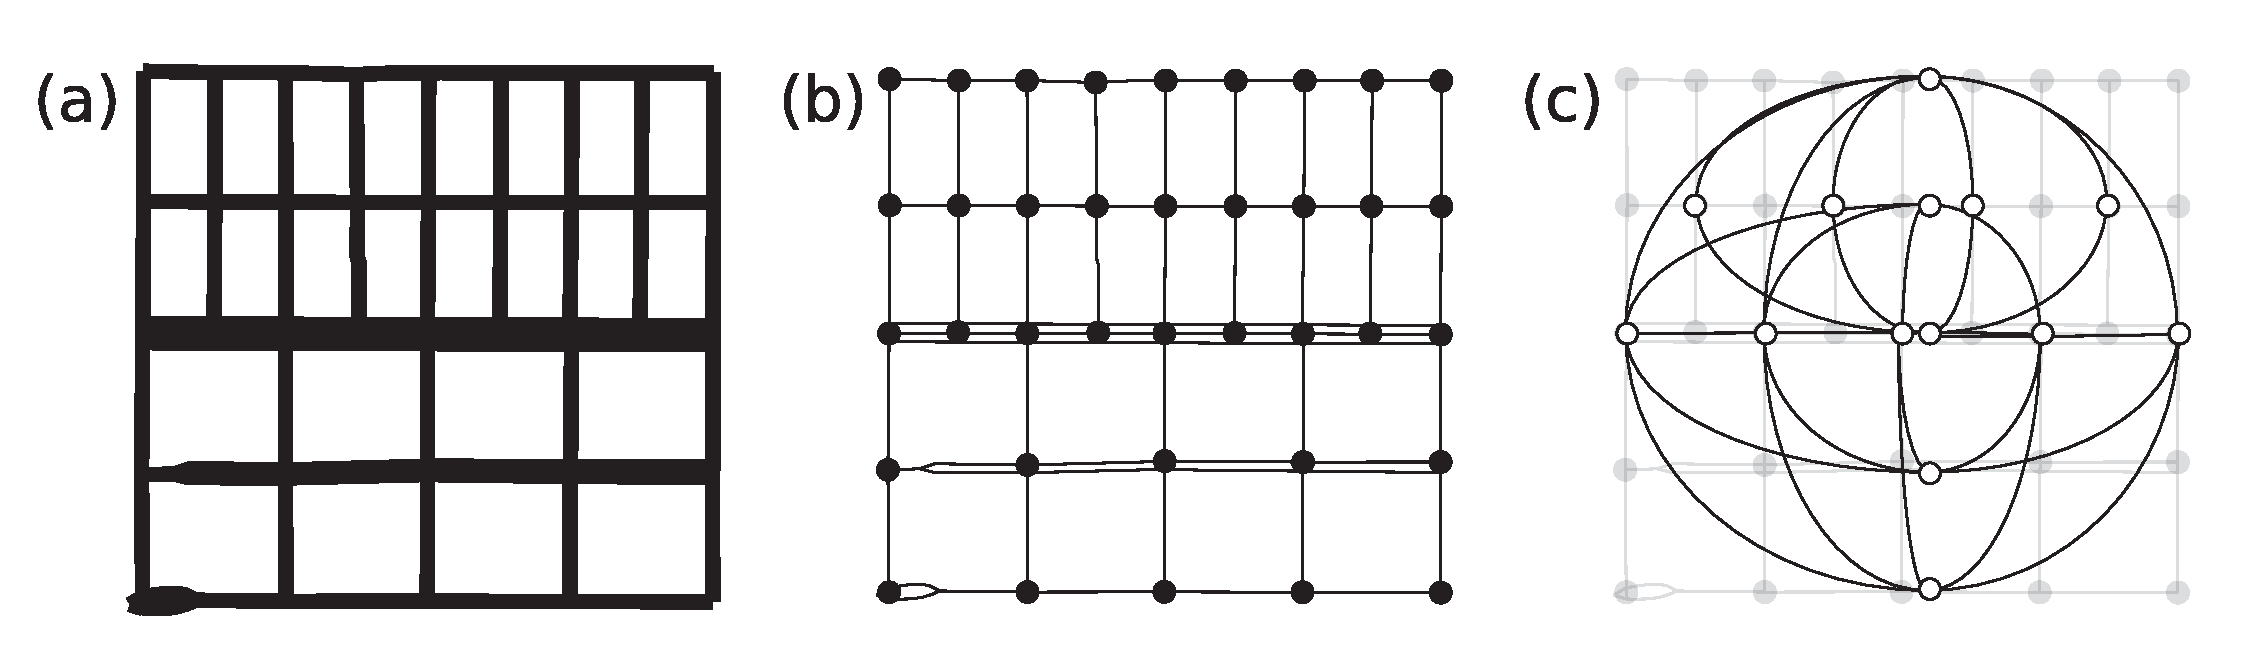
\includegraphics[width=\textwidth]{images/introduction/networks.pdf}
	\caption[Network representation of a city]{\textbf{(a)} Schematic street plan representation. \textbf{(b)} Primal representation of a street network, intersections are represented as nodes, and streets as edges. \textbf{(c)} Space syntax representation of a city. Continues streets mapped as nodes, and edges between intersecting streets.}
	\label{fig:networks}
\end{figure*}

%Street networks
When thinking of a city as a network, there are two approaches: First, map the intersections as nodes, the streets (or any other mobility infrastructure) as edges~\cite{porta2006primal}. Following this approach it is possible to replicate the city's structure as a planar network~\cite{Boeing2020Planarity} (see Figure~\ref{fig:networks}~(a-b)). On the other hand, it is possible to model a city as a network following space syntax theory~\cite{hillier1976syntax} in which the streets are mapped as nodes depending on their continuity, and intersections are edges (see Figure~\ref{fig:networks}~(c)). Although, the space syntax theory is useful to map relations between spaces/streets, it came short to capture the morphological properties of cities~\cite{batty2004new}. Along this thesis we will work with the primal representation of urban networks, considering intersections as nodes, and streets, sidewalks, bike paths as edges connecting the nodes.

%Multimodal transportation and networks

%Mobility and networks
The complex system of urban transport infrastructure is shaping the dynamics of human mobility, a network embedded in space with special properties. The availability of data sets on urban infrastructure networks has enabled first insights into the topological constraints on human movements. Large-scale mobile phone data sets, on the other hand, have been used as proxies to understand mobility patterns in cities~\cite{gonzalez2008understanding}, finding predictable human mobility motifs related to socio-economic activities in cities. The use of such massive data sets has also provided insights into the possibilities of shareability, and into the efficient allocation of space for different types of transportation.

%State research problems

\section{Aim and structure of the thesis}

The primary aim of this thesis is to contribute to the better understanding of the structural properties of multimodal transportation networks in urban areas. For that, we build on the tools and methods of network science to analyze the underlying complexity of urban mobility infrastructure. 

We begin focusing on the multimodal infrastructure network, first by providing a review of previous works related to multimodal transportation networks, and then giving an original contribution to the analysis of this specific type of system. In the following chapters, we focus the attention to specific layers: first, by analyzing and giving an original contribution for the connectivity of bicycle infrastructure networks, second, we propose and use a methodology to measure the urban quality of life as urban walkability taking the pedestrian infrastructure layer as the base for our calculations.

This thesis is structured as follows:

\begin{itemize}
    \item Chapter~\ref{ch:litReview}: We provide a review of previous works on multimodal transportation and mobility research from a complex systems' perspective. First we focus on the infrastructure and measures to quantify it, then on the mobility dynamics on top of these infrastructures, and finally we offer a review of available datasets and tools to analyze this specific type of networks.
    \item Chapter~\ref{ch:OverlapCensus}: We make an original contribution to the field by proposing a method to extract the multimodal profile from a city's multiplex transport network. In this chapter, we apply our methods to fifteen cities, finding clusters of cities with similar multimodal infrastructure.
    \item Chapter~\ref{ch:BikeGrowth}: We focus our attention in the bicycle layer of the multimodal network and propose algorithmic approaches to improve its connectivity. We find that focalized investment has the potential to rapidly improve the connectedness and directness of the bicycle infrastructure.
    \item Chapter~\ref{ch:LQI}: We present a methodology to measure the quality of life in a city based on the pedestrian accessibility to amenities and services. We apply the methodology to Budapest and show how it can be used to capture inequalities in neighborhoods. 
    \item Chapter~\ref{ch:Conclusion}: We review the main contributions from this thesis, and outline future streams of work and open questions. 
\end{itemize}

% Introduction structure:  

% - Introduction to topic and its context, narrowing it down to identifying a research problem  

% - literature review on the research problem (what is known), and possible contribution (what is not known / how you can add to existing knowledge)  

% - the purpose of your research (purpose statment / research question) 

% - methodology of your research  

% - dissertation structure map (what you do in each chapter)  